\chapter{Basistechnologien}
\thispagestyle{standard}
\pagestyle{standard}
\renewcommand{\footrulewidth}{0.4pt}
\lfoot{\small Refik Kerimi}

\section{Aufbau PWA}
In diesem Kapitel werden die Komponenten der \acl{PWA} (\cite{PWA}) allgemein erklärt. Weiter werden durch die Tabelle \ref{tab:PwaNvaWa} die wichtigsten Punkte gegenübergestellt.  
\begin{figure}[h]
	\centering
	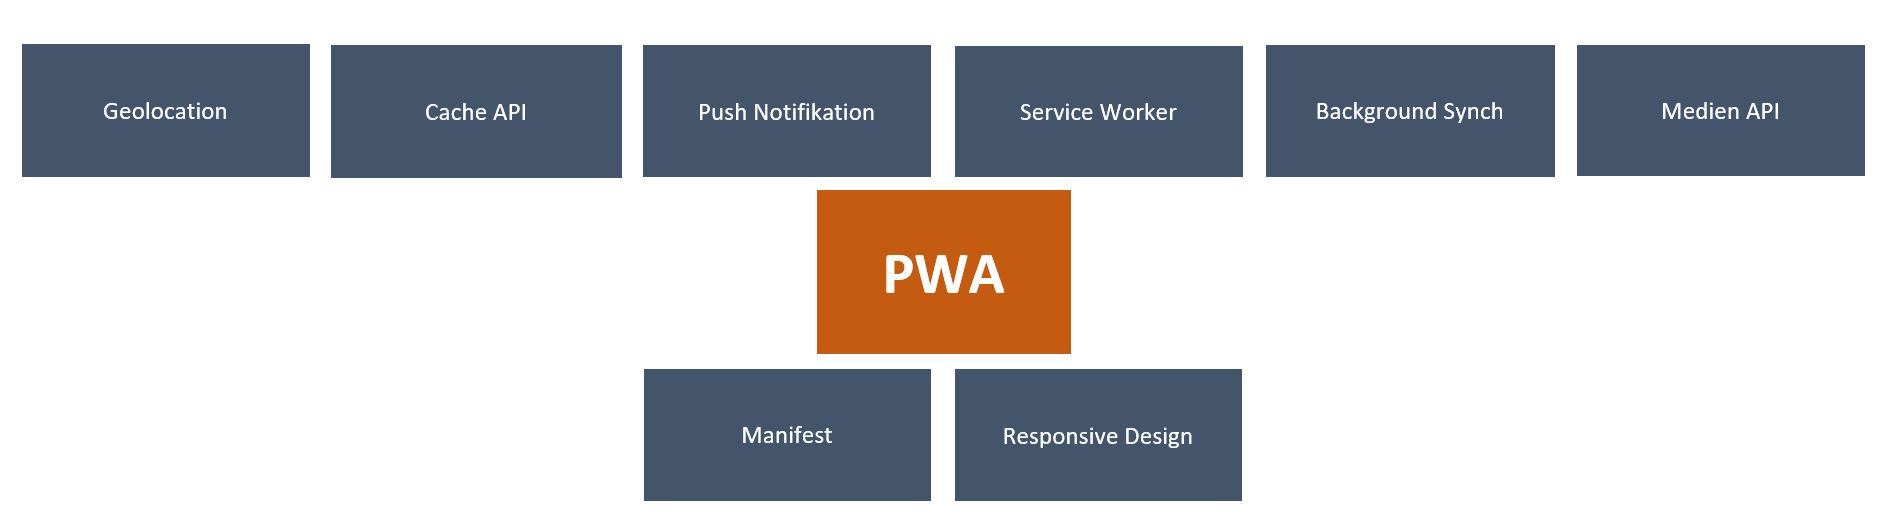
\includegraphics[width=14cm]{BilderAllgemein/PWA_Features}\medskip
	\caption{PWA Komponenten}
	\label{fig:Komponenten}
\end{figure}

\section{PWA vs. Native APP vs Wep APP}
Folgende Punkte werden gegenübergestellt:
\begin{itemize}
    \item  \textbf{Veröffentlichung und Installation}
	\item  \textbf{Zugriff}
	\item  \textbf{Funktionen}
\end{itemize}. 

\begin{table}[h]
\centering

\begin{tabular} {|p{3cm}|p{3.5cm}|p{3.5cm}|p{3.5cm}|}
\hline\multirow{3}{*}
 										&PWA  & Native & Web App	\\ \hline
Veröffentlichung & Es werden verschiedene Entwicklerkonten benötigt Play Store und Apple Store & keine Entwicklerkonten benötigt & keine Entwicklerkonten benötigt\\ \hline

Installation & App muss aus einem der App-Stores downgeloaded werden  & Wird mit einem Klick auf dem Startbildschirm hinzugefügt & keine Funktion\\ \hline

Updates &  über App-Store & Sofortige Updates & Sofortige Updates\\ \hline


   				  						 
				
\end{tabular}    
\caption{Veröffentlichung und Installation \cite{PwaNvaWa}}
\label{tab:PwaNvaWa}
\end{table}


\begin{table}[h]
\centering

\begin{tabular} {|p{3cm}|p{3.5cm}|p{3.5cm}|p{3.5cm}|}
\hline\multirow{3}{*}
 										&PWA  & Native & Web App	\\ \hline
Offline-Zugriff & Verfügbar & Man muss die App einmal online nutzen, dann sollten die Inhalte im Cache offline verfügbar sein. & nicht möglich\\ \hline

starten im Vollbildmodus & möglich  & möglich & nicht möglich\\ \hline

Kundenbindung &  sehr Hoch, Kunden verbringen viel Zeit & App ist wie ein Tap, dass macht es für den Kunden leichter zu Wechseln & wie \acs{PWA}\\ \hline


   				  						 
				
\end{tabular}    
\caption{Zugriff \cite{PwaNvaWa}}
\label{tab:PwaNvaWa}
\end{table}

%Tabelle verwenden
%https://apptooltester.com/de/progressive-web-%apps/

 \newpage



\section{Web App Manifest}
Das App Manifest ist ein JSON File verrät dem Browser wie sich die \acs{WA}, bei der Installation auf dem Startbildschirm, verhält. Im Manifest wird der Name,der Kurzname, die Größe, Aussehen der Icons und weitere Eigenschaften definiert diese im Kapitel \ref{chap:Entwurf} näher erklärt werden.


\subsection{Bereitstellung des Web App Manifest}
das App Manifest.json file wird in die gleiche Ebene wie die Index.html Datei in das Projekt eingepflegt und und übre den folgenden Link-Tag in der Index Datei bereitgestellt:


\begin{lstlisting}[language=HTML, caption={Manifest.json},label=lst:Manifest.json, xleftmargin=50pt]
<link rel="manifest" href="/<Dateinname>">
\end{lstlisting}

\newpage
Der Aufbau der Manifest ist wie in Listening (Nr) gezeigt aufgebaut:
\begin{lstlisting}[language=json, firstnumber=1, caption={Manifest in das Projekt implementieren},label=lst:Manifest.json, xleftmargin=50pt]
{
  "name": "HackerWeb",
  "short_name": "HackerWeb",
  "start_url": ".",
  "display": "standalone",
  "background_color" : "#fff" ,
  "description": "Eine einfach lesbare Hacker News App.",
  "Icons": [{
    "src": "images/touch/homescreen48.png",
    "sizes": "48x48",
    "type": "image/png"
  }, {
    "src": "images/touch/homescreen72.png",
    "sizes": "72x72",
    "type": "image/png"
  }, {
    "src": "images/touch/homescreen96.png",
    "sizes": "96x96",
    "type": "image/png"
  }, {
    "src": "images/touch/homescreen144.png",
    "sizes": "144x144",
    "type": "image/png"
  }, {
    "src": "images/touch/homescreen168.png",
    "sizes": "168x168",
    "type": "image/png"
  }, {
    "src": "images/touch/homescreen192.png",
    "sizes": "192x192",
    "type": "image/png"
  }],
  "related_applications": [{
    "platform": "Web"
  }, {
    "platform": "play",
    "url": "https://play.google.com/store/apps/details?id=cheeaun.hackerweb"
  }]
}
\end{lstlisting}\cite{Manifest}

\subsection{Zum Startbildschirm hinzufügen}
Um den Banner am Mobilen Gerät anzuzeigen müssen folgende Kriterien erfüllt werden:


\begin{itemize}
    \item  die App ist noch nicht installiert
	\item  min 30 Sekunden lang mit der Domäne interagiert
	\item  beinhaltet ein Web App Manifest mit folgenden Werten:
		 \begin{itemize}
         \item Kurzname oder Name
         \item icons - muss ein 192px und ein 512px großes Icon enthalten
         \item Startadresse
         \item Anzeige muss eines der folgenden sein: fullscreen, standalone oder minimal-ui
      	\end{itemize}
    \item 	darf nur über HTTPS aufrufbar sein
    \item beinhaltet einen \acl{SW} mit einem Fetch-Event-Handler
\end{itemize}

Wenn diese Punkte erfüllt sind startet Chrome ein beforinstallprompomt wie in Listen(refereiniziern):

\begin{lstlisting}[language=JavaScript, caption={beforinstallprompt},label=lst:beforinstallprompt, xleftmargin=50pt]
let deferredPrompt;

window.addEventListener('beforeinstallprompt', (e) => {
  // Prevent Chrome 67 and earlier from automatically showing the prompt
  e.preventDefault();
  // Stash the event so it can be triggered later.
  deferredPrompt = e;
});
\end{lstlisting}



\section{Service Worker}
%\label{sec:Service Worker} zuweisung zu anderen Sektor
Der \acl{SW} (\acs{SW}) ist ein Script das der Browser im Hintergrund ausführt \cite{ServiceWorkerRegistration}. Mit der Hilfe des \acs{SW} ist es möglich die \acs{WA} offline zu betreiben, Push Notifikation zu erhalten, gecachte Daten abzurufen. \acs{SW} verhalten sich wie Proxy-Server, welche in einer Zwischenschicht vom Browser und den Netzwerk sitzen. 
Ein \acs{SW} wird von einem Worker-Kontext \cite{Worker} ausgeführt, hat keinen DOM Zugriff und wird als Haupt-Java Script Thread verwendet \cite{ServiceWorker}.

\subsection{Basis Architektur}
Der Cyclus eines \acs{SW}s ist von der Webseite getrennt.
In der Installationsphase werden benötigte statische Datein zwischengespeichert erst danach ist der \acs{SW} installiert. Die Installation erfolgt über die JavaScript-Funktion:

\begin{lstlisting}[language=JavaScript, caption={Service Worker Navigator},label=lst:ServiceWorkerNavigator, xleftmargin=50pt]
navigator.serviceWorker.register
\end{lstlisting}

Danach folgt die Aktivierungsphase, in dieser Phase werden alte Cache-Inhalte verwaltet und Aktualisiert.


\begin{figure}[h]
	\centering
	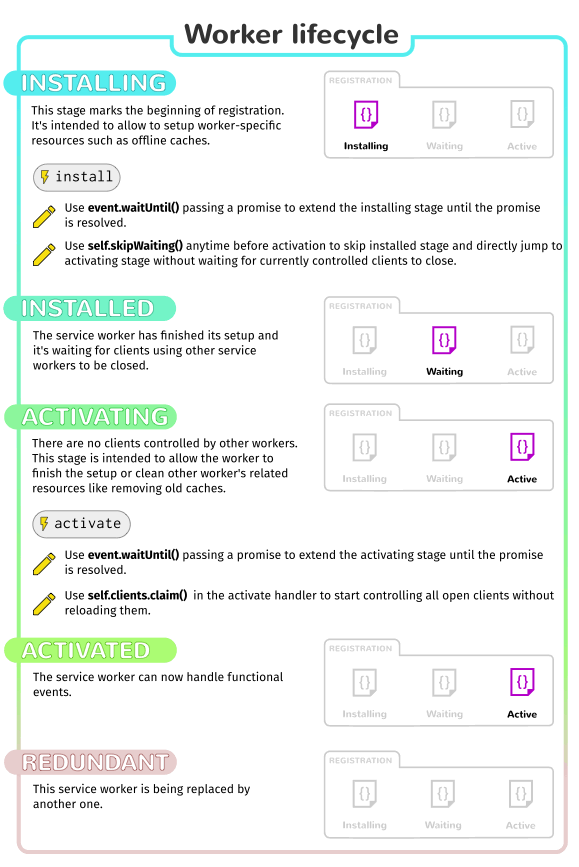
\includegraphics[width=6cm]{BilderAllgemein/swLifecycle}\medskip
	\caption{Basis Architektur \acl{SW}}
	\label{fig:Erstinstallation}\cite{ServiceWorkerArchitecture}
\end{figure}
Um die neuen Seiten zu steuern muss der \acs{SW} erneut geladen werden.
In der Abbildung \ref{fig:Erstinstallation} ist eine vereinfachte Erstinstallation zu sehen:

\newpage
\subsection{Registrierung Service Worker}\label{chap:RegistrierungServiceWorker}

Um den \acs{SW} zu registrieren muss folgender \acs{JS}-Code in das Projekt im (genauen Pfad rausfinden) integriert werden.
\begin{lstlisting}[language=JavaScript, caption={Service Worker Register},label=lst:ServiceWorkerRegister, xleftmargin=50pt]
if ('serviceWorker' in navigator) {
  window.addEventListener('load', function() {
    navigator.serviceWorker.register('/sw.js').then(function(registration) {
      // Registration was successful
      console.log('ServiceWorker registration successful with scope: ', registration.scope);
    }, function(err) {
      // registration failed :(
      console.log('ServiceWorker registration failed: ', err);
    });
  });
}
\end{lstlisting}

Hier wird die Unterstützung durch den Browser geprüft.


\begin{figure}[h]
	\centering
	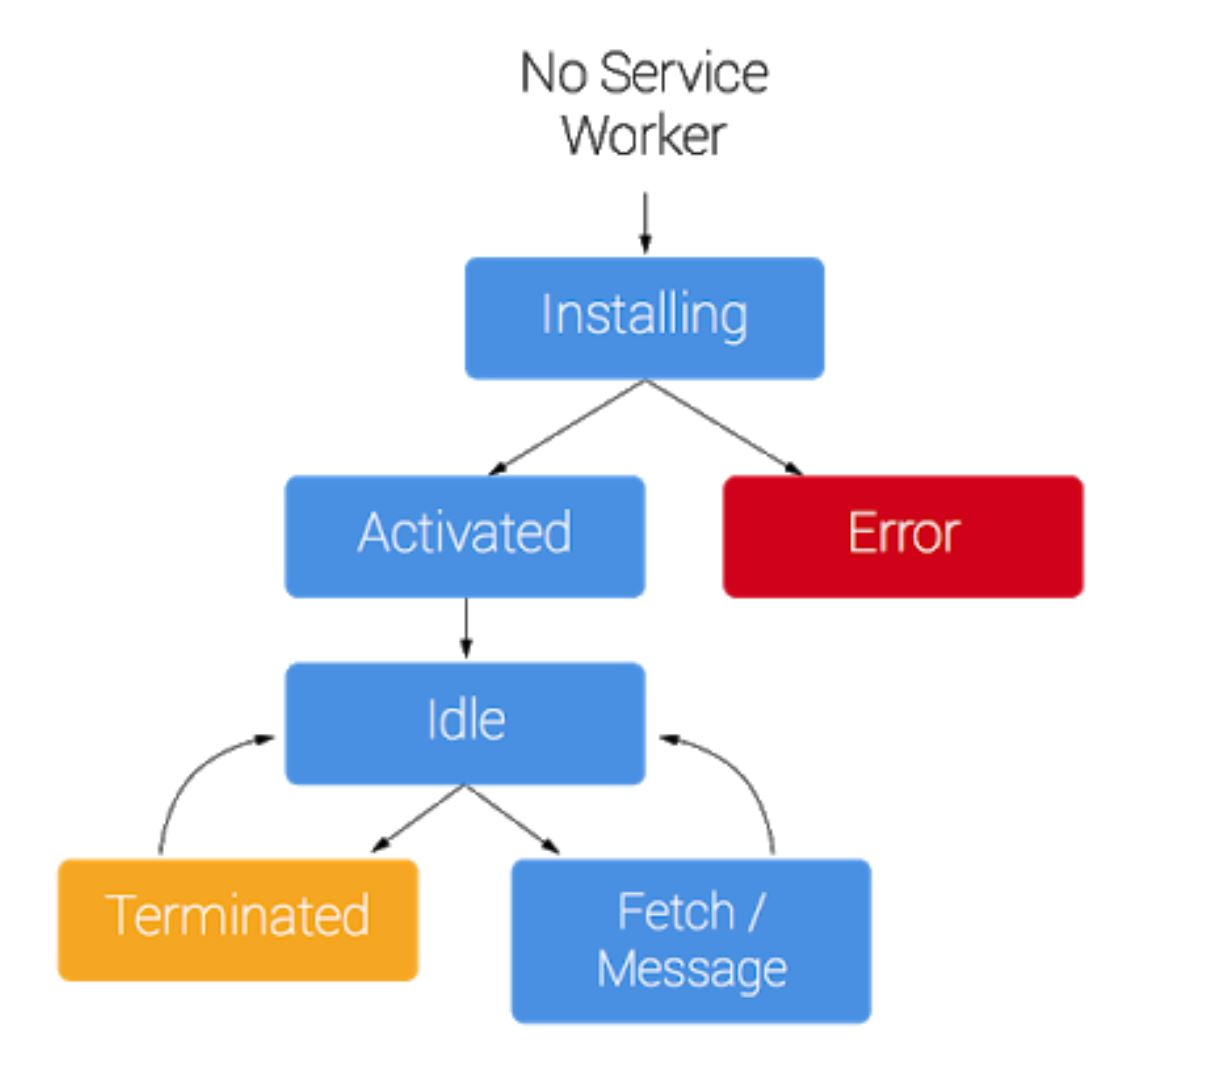
\includegraphics[width=8cm]{BilderAllgemein/InstallSW}\medskip
	\caption{Erstinstallation Service Worker}
	\label{fig:Erstinstallation}\cite{ServiceWorkerRegistration}
\end{figure}

Der \acs{SW} kann nach der Übernahme der Steuerung zwei Zustände übernehmen, entweder dieser wird beendet oder er übernimmt die Verwaltung der Netzwerkanfragen und der Nachrichten \cite{ServiceWorkerRegistration}.



\subsection{Cache API}
Die \acs{SW} API stellt ein Cache-Schnittstelle zum speichern von Daten auf dem Browser über IndexDB \cite{IndexDB} gespeichert und können auch wieder bei bedarf aufgerufen werden. Die API wurde ursprünglich für den \acs{SW} entwickelt, diese kann aber von jedem Script verwendet werden. 
Wie die API gestaltet wird, hängt ganz von den Anforderungen der Applikation ab.
Der Einstiegspunkt ist 'cache' wie man im folgenden Codebeispiel sehr gut erkennen kann.

\begin{lstlisting}[language=JavaScript, caption={Service Worker Cache},label=lst:ServiceWorkerCache, xleftmargin=50pt, label=cache]
self.addEventListener('install', function(event) {
  event.waitUntil(
    caches.open(cacheName).then(function(cache) {
      return cache.addAll(
        [
          '/css/bootstrap.css',
          '/css/main.css',
          '/js/bootstrap.min.js',
          '/js/jquery.min.js',
          '/offline.html'
        ]
      );
    })
  );
});
\end{lstlisting}

Im Listening \ref{list:cache} zu sehen werden statische HTML, CSS und JS Dateien gecacht bevor der intall event des \acs{SW} aufgerufen wird. Die Callbackfunktion ruft die Cache-API auf \cite{CacheAPI}.
Um den Event Aufzurufen werden Promises für Asynchrone Aufrufe verwendet \cite{Promises}.
Es gibt wie in \cite{CacheAPI} beschrieben noch andere Möglichkeiten um die Cache API nützlich in ein Projekt einzubauen.
\newpage

\section{Push Notifikation}
Um dem User bei einer \acs{PWA} das Gefühl einer Native App aufkommen zu lassen ist die Push Funktion unablässig. Erst durch diese Funktion in Kombination mit dem \acs{SW} gibt der \acl{WA} die persönliche Nähe zum User \cite{PushNotifikation}.



\subsection{Registrierung Push Notifikation}
Um die Push Funktion zu integrieren muss die Registerfunktion des \acs{SW} wie folgt erweitert werden:
 
\begin{lstlisting}[language=JavaScript, caption={Push Notifications},label=lst:PushNotifikation, xleftmargin=50pt]
if ('serviceWorker' in navigator && 'PushManager' in window) {
  console.log('Service Worker and Push is supported');

  navigator.serviceWorker.register('sw.js')
  .then(function(swReg) {
    console.log('Service Worker is registered', swReg);

    swRegistration = swReg;
  })
  .catch(function(error) {
    console.error('Service Worker Error', error);
  });
} else {
  console.warn('Push messaging is not supported');
  pushButton.textContent = 'Push Not Supported';
}
\end{lstlisting}

Hier wird der Support der Pushfunktionen durch den Browser überprüft wie in \\ Kapitel \ref{chap:RegistrierungServiceWorker} die Browserunterstützung vom \acs{SW} und die Push Benachrichtigung. Bei fehlerlosen Durchlauf wird die \acs{SW}.js Datei registriert \cite{PushNotifikation}.

\newpage



\subsection{Geolocation}
https://appdevelopermagazine.com/5877/2018/3/1/progressive-web-apps-vs-native-apps:-showdown-in-2018/


\subsection{Camera API}


\subsection{Browser} 





